\documentclass[aspectratio=169]{beamer}

\usepackage[utf8]{inputenc} 
\usepackage[T1]{fontenc}
\usepackage{lmodern}
\usepackage{graphicx}
\usepackage[french]{babel}
\usepackage{vwcol}
\usepackage{listings}
\usepackage{color}
\usepackage{impnattypo}
\usepackage[export]{adjustbox}

\usefonttheme{serif}

\title{Soutenance dossier professionnel}
\author{Geoffrey Brunet}
\institute{EPSI Auxerre | Quartz-Insight}

\usetheme{Frankfurt}
\makeatletter
\setbeamertemplate{headline}

\begin{document}

\maketitle

\AtBeginSection[]{
    \begin{frame}
        \begin{center}{\Large Plan }\end{center}
        \tiny{\tableofcontents[currentsection, hideothersubsections]}
    \end{frame}
}

\section{Présentation personnelle et de l'entreprise}

\begin{frame}
    \frametitle{Présentation personelle}
    \begin{columns}
        \begin{column}{0.5\textwidth}
            \begin{itemize}
                \item Passioné d'informatique
                \item Développeur en alternance
                  depuis 3 ans
                \item Études à l'EPSI
                \item Sciences, trail, tatouages,
                  photographie argentique
            \end{itemize}
        \end{column}
        \begin{column}{0.5\textwidth}
            
\includegraphics[height=0.20\textheight]{Imgs/logo-epsi-v2.png}
        \end{column}
    \end{columns}
\end{frame}

\begin{frame}
    \frametitle{Présentation de l'entreprise}
    \begin{columns}
        \begin{column}{0.5\textwidth}
            
\includegraphics[height=0.20\textheight]{Imgs/logo-quartz-insight-v2.png}
        \end{column}
        \begin{column}{0.5\textwidth}
            \begin{itemize}
                \item Création en 2013
                \item Cabinet de conseils
                \item Business Intelligence
                \item Entreprise Performance Management
                \item R\&D bases de données multidimensionnelles
            \end{itemize}
        \end{column}
    \end{columns}
\end{frame}

\begin{frame}
    \frametitle{Organigramme de Quartz-Insight}
    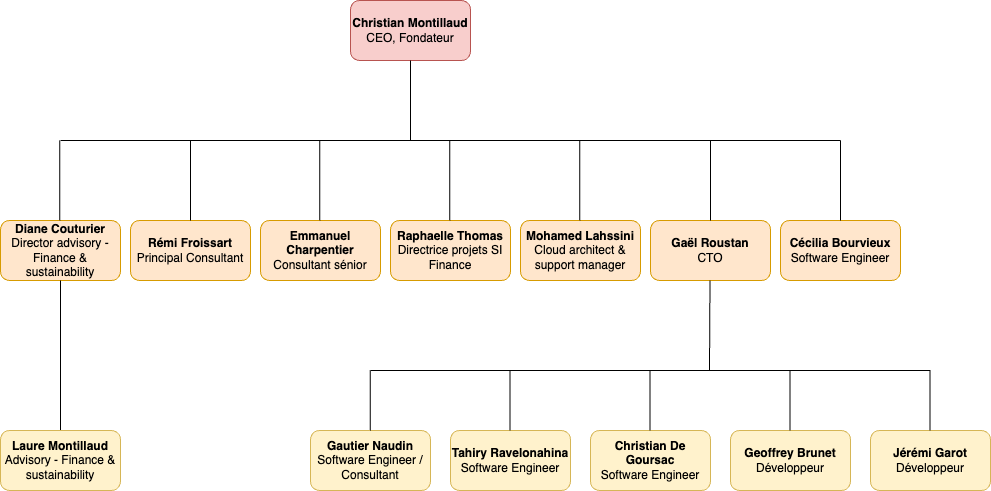
\includegraphics[height=0.56\textheight]{Imgs/organigramme-quartz-insight.png}
\end{frame}

\begin{frame}
    \frametitle{Présentation du projet}
    \begin{columns}
        \begin{column}{0.5\textwidth}
            \begin{itemize}
              \item Refonte en microservices
              \item Normalisation des technologies
              \item Ajout de nouvelles fonctionnalitées
              \item Amélioration de l'UX/UI
            \end{itemize}
        \end{column}
        \begin{column}{0.5\textwidth}
            
\includegraphics[height=0.40\textheight]{Imgs/dotnet-core.png}
        \end{column}
    \end{columns}
\end{frame}

\section{Activités et compétences}

\begin{frame}
  \frametitle{1. Cartographie complète du système d’information existant}
  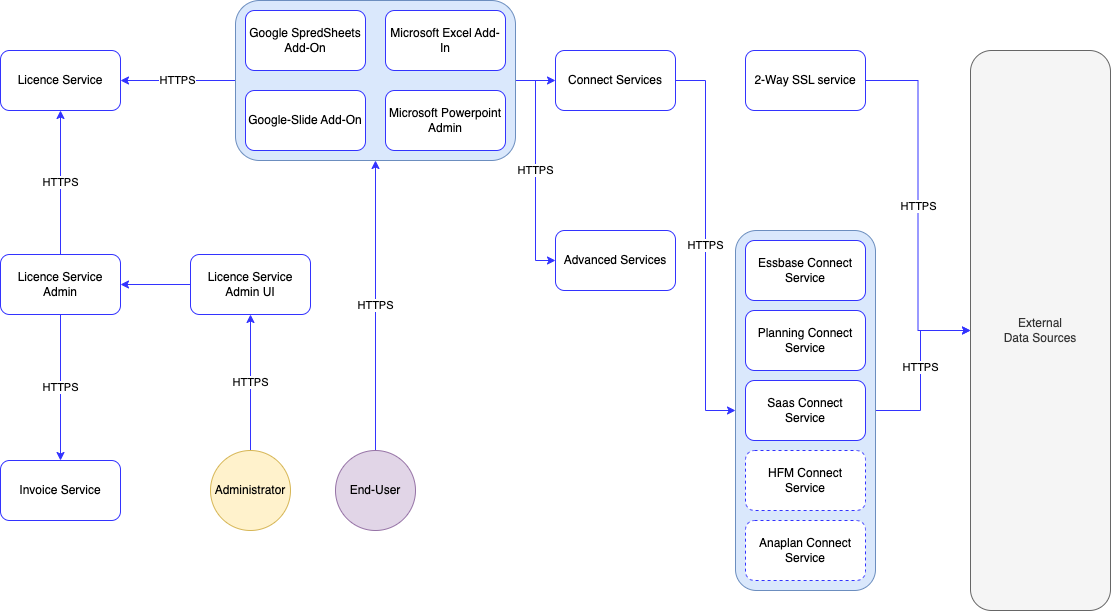
\includegraphics[height=0.60\textheight]{Imgs/schema-qibates-original.png}
\end{frame}

\begin{frame}
  \frametitle{2. Cartographie des informations sensibles, 
  évaluation des risques et définition d’une politique de sécurité}
  \begin{columns}
    \begin{column}{0.5\textwidth}
      \begin{itemize}
        \item Analyse des points chauds
        \item Réalisation d'un PSSI
        \item Norme ISO 27001
        \item 3 axes à suivre: confidentialité, intégrité et disponibilité
      \end{itemize}
    \end{column}
    \begin{column}{0.5\textwidth}
      
\includegraphics[height=0.50\textheight]{Imgs/anssi.png}
    \end{column}
  \end{columns}
\end{frame}

\begin{frame}
  \frametitle{3. Analyse des données de références pour la création d’un référentiel de données}
  \begin{columns}
    \begin{column}{0.5\textwidth}
      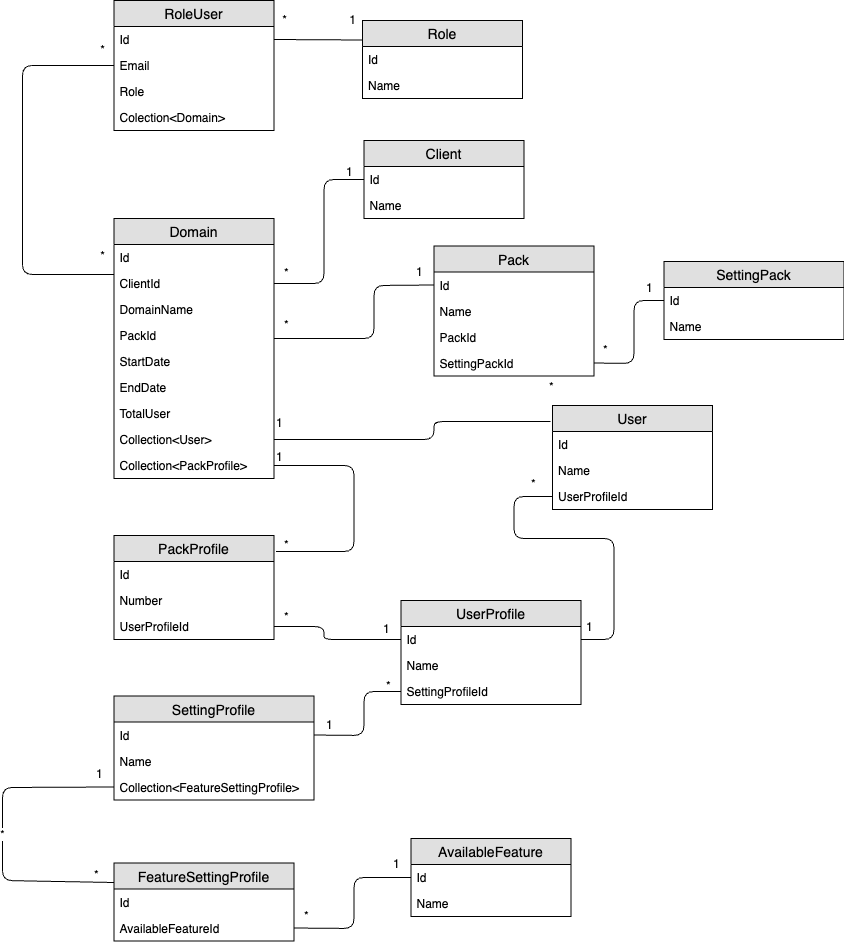
\includegraphics[height=0.65\textheight, center]{Imgs/ralph-diagram.png}
    \end{column}
    \begin{column}{0.5\textwidth}
      \begin{itemize}
        \item Recherche du SGBD et de la BDD
        \item Analyse de la BDD (recherche et compréhension des tables)
        \item Réalisation d'un MCD
      \end{itemize}
    \end{column}
  \end{columns}
\end{frame}

\begin{frame}
  \frametitle{4. Analyse des besoins métiers pour une solution applicative sur mesure}
  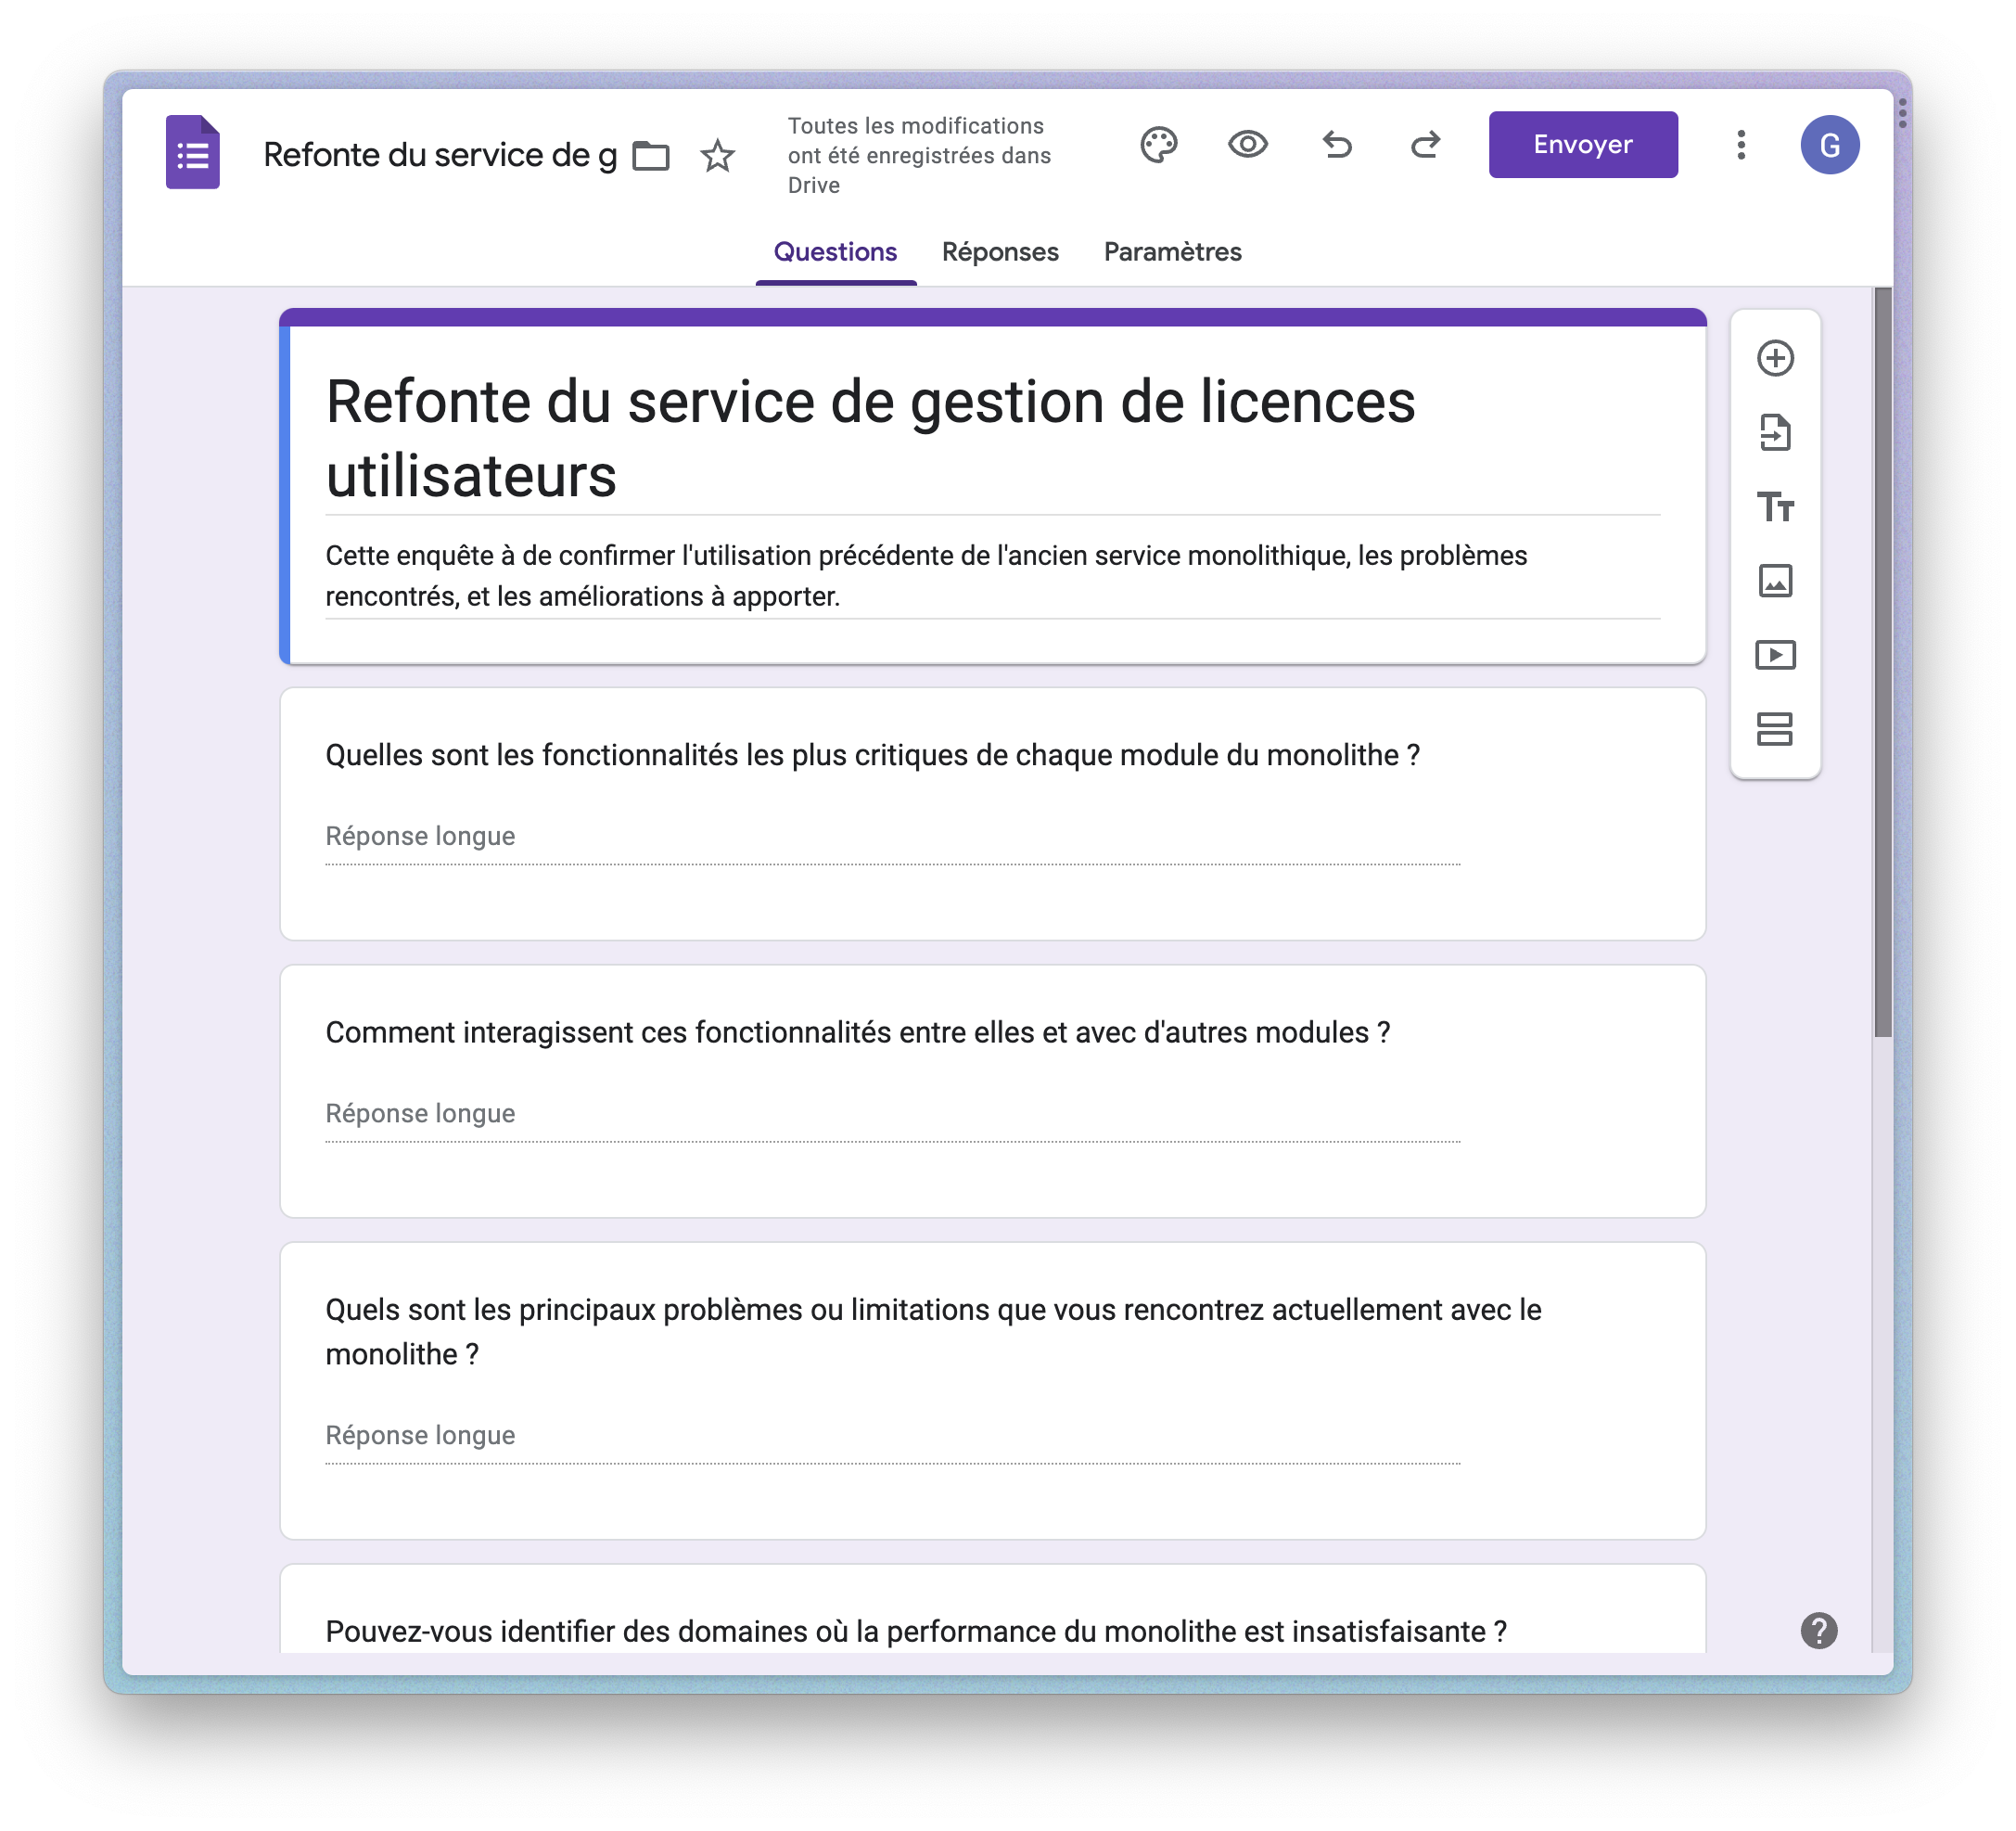
\includegraphics[height=0.80\textheight, center]{Imgs/enquete-utilisateur.png}
\end{frame}

\begin{frame}
  \frametitle{5. Conception d’une architecture applicative évolutive et tolérante aux pannes}
  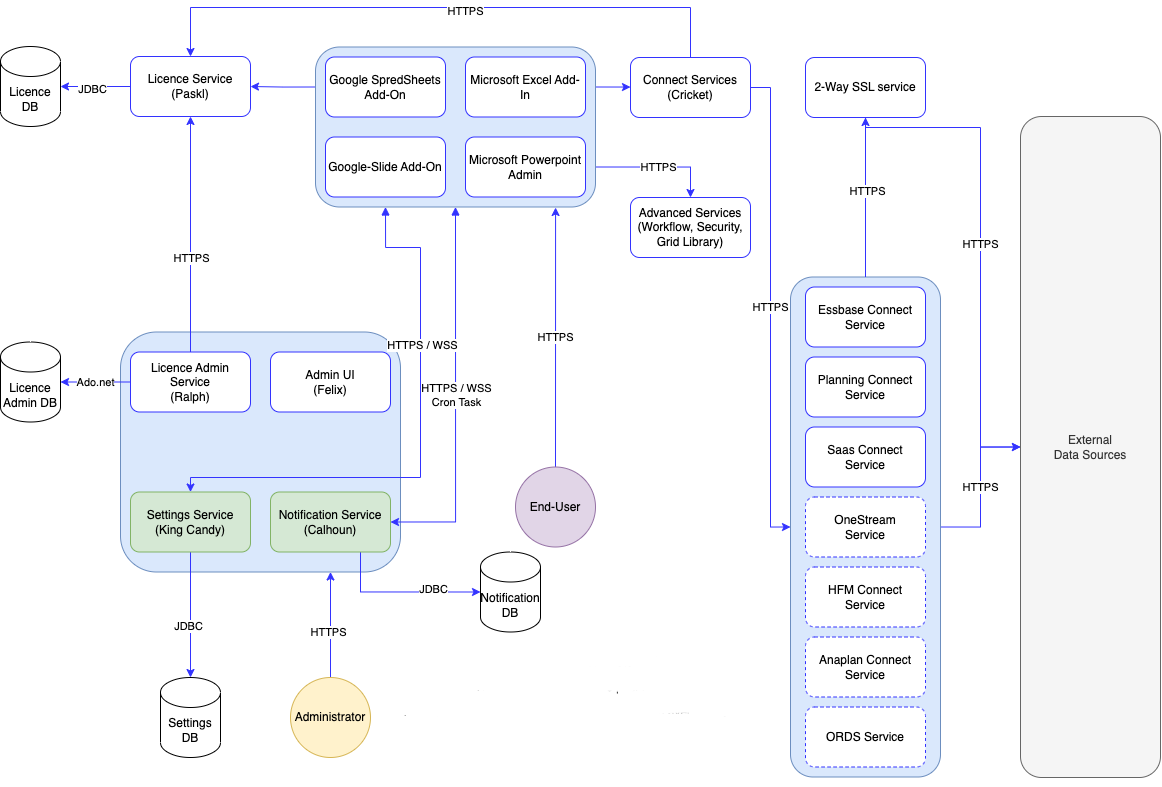
\includegraphics[height=0.75\textheight, center]{Imgs/schema-qibates-v2.png}
\end{frame}

\begin{frame}
  \frametitle{6. Développement d’une application pour répondre aux besoins utilisateurs/directions métiers}
  \begin{columns}
    \begin{column}{0.5\textwidth}
      \begin{itemize}
        \item Choix des technologies
        \item Développement des microservices (TDD)
        \item une application web et trois API REST 
      \end{itemize}
    \end{column}
    \begin{column}{0.5\textwidth}
      
\includegraphics[height=0.75\textheight, center]{Imgs/icons.png}
    \end{column}
  \end{columns}
\end{frame}

\begin{frame}
  \frametitle{6. Développement d’une application pour répondre aux besoins utilisateurs/directions métiers}
  \begin{columns}
    \begin{column}{0.5\textwidth}
      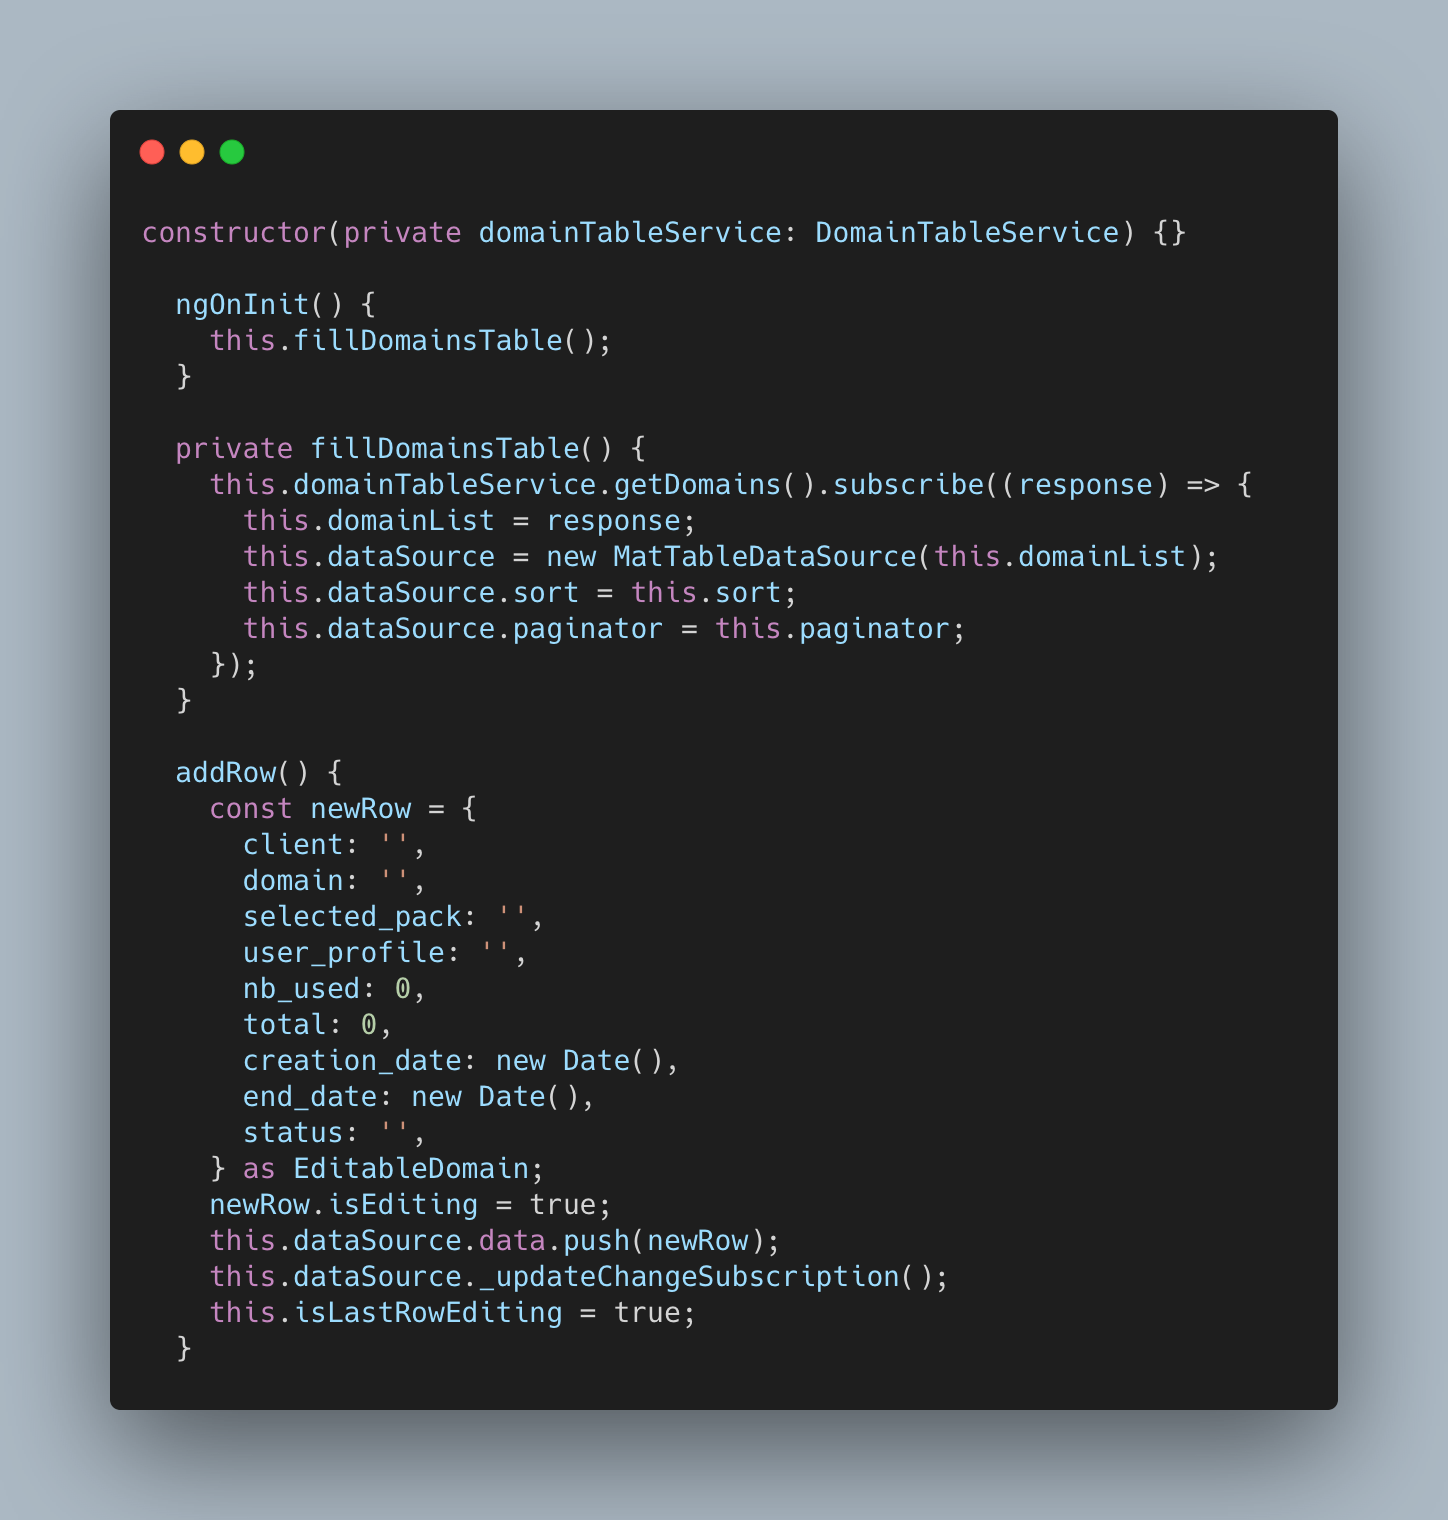
\includegraphics[height=0.50\textheight, center]{Imgs/js-code.png}
    \end{column}
    \begin{column}{0.5\textwidth}
      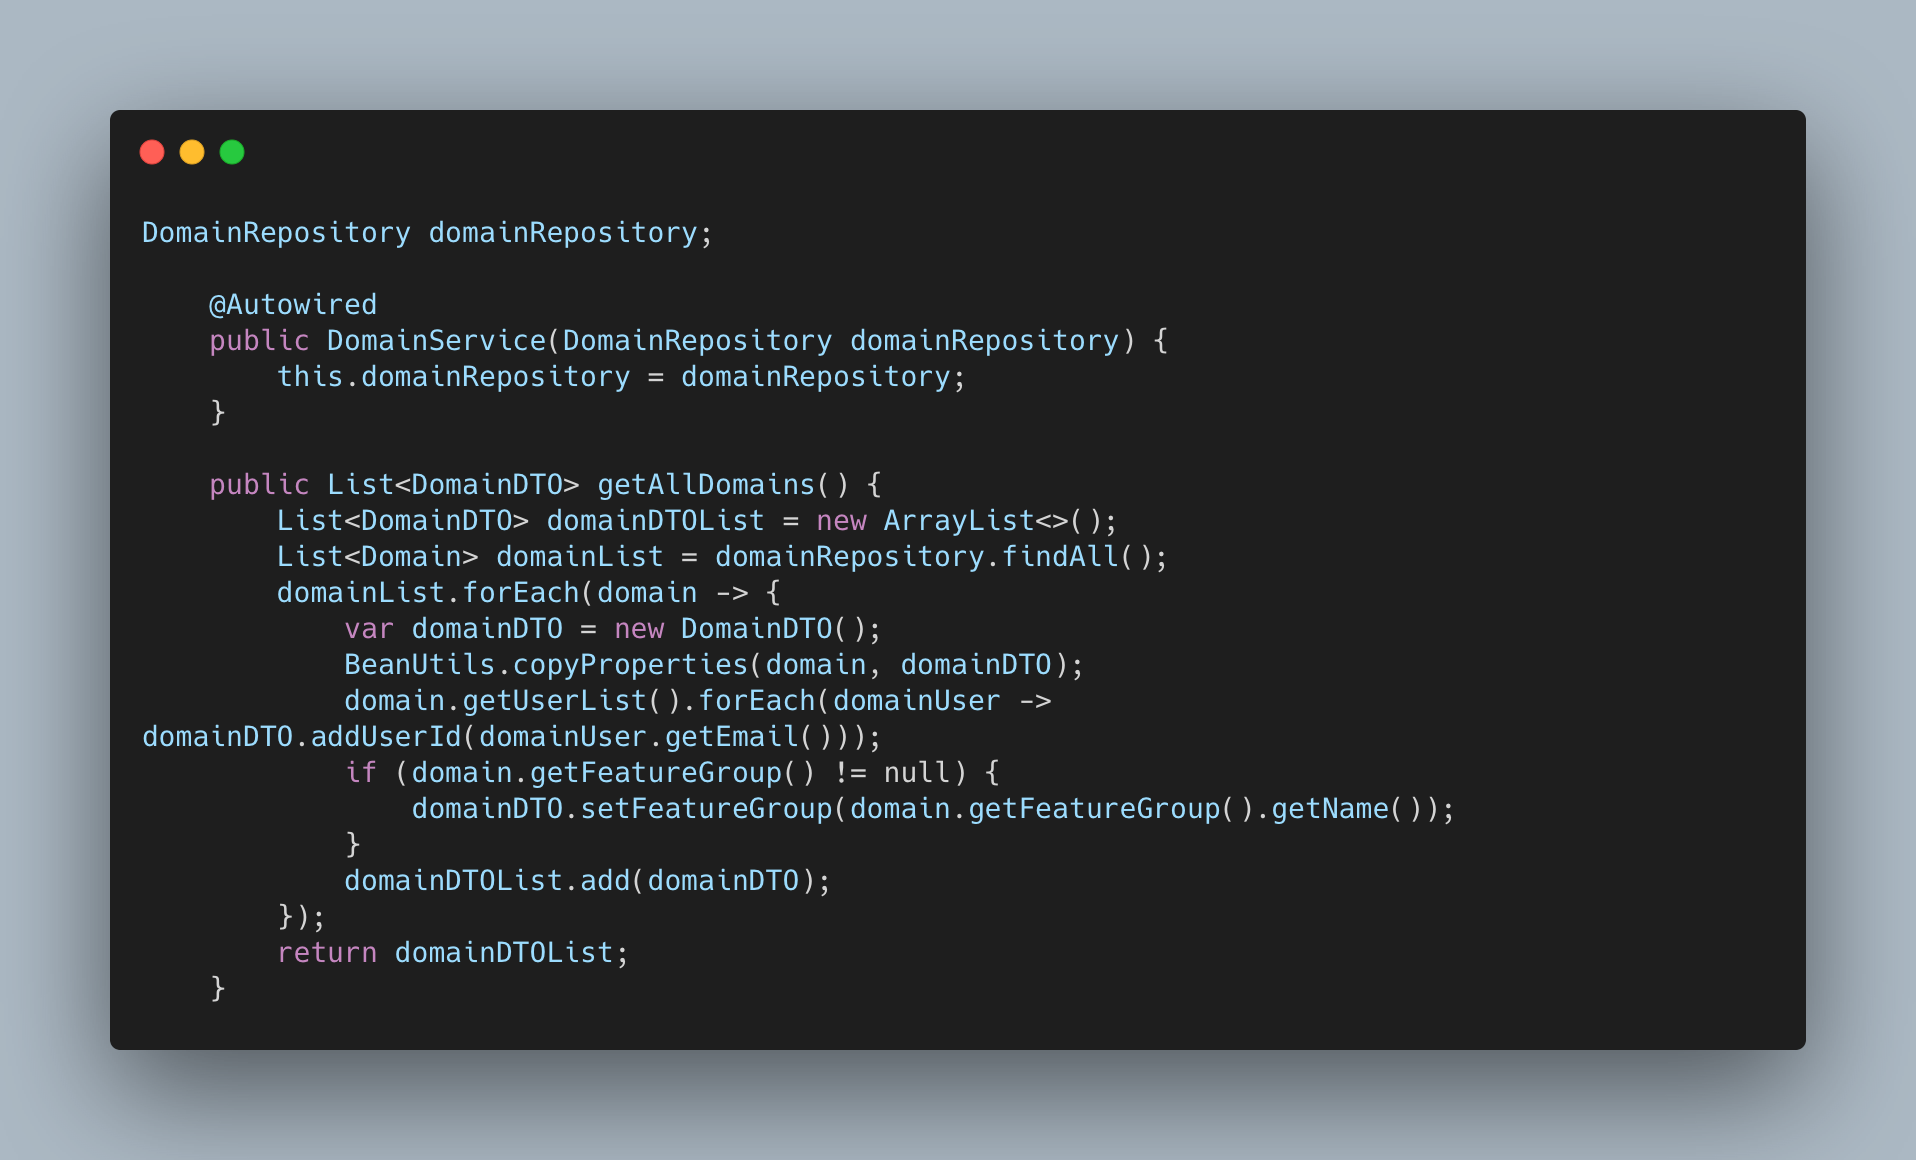
\includegraphics[height=0.50\textheight, center]{Imgs/java-code.png}
    \end{column}
  \end{columns}
\end{frame}

\begin{frame}
  \frametitle{7. Analyse de la qualité de la solution applicative et mise en place d’un plan de correction / d’amélioration}
  \begin{columns}
    \begin{column}{0.5\textwidth}
      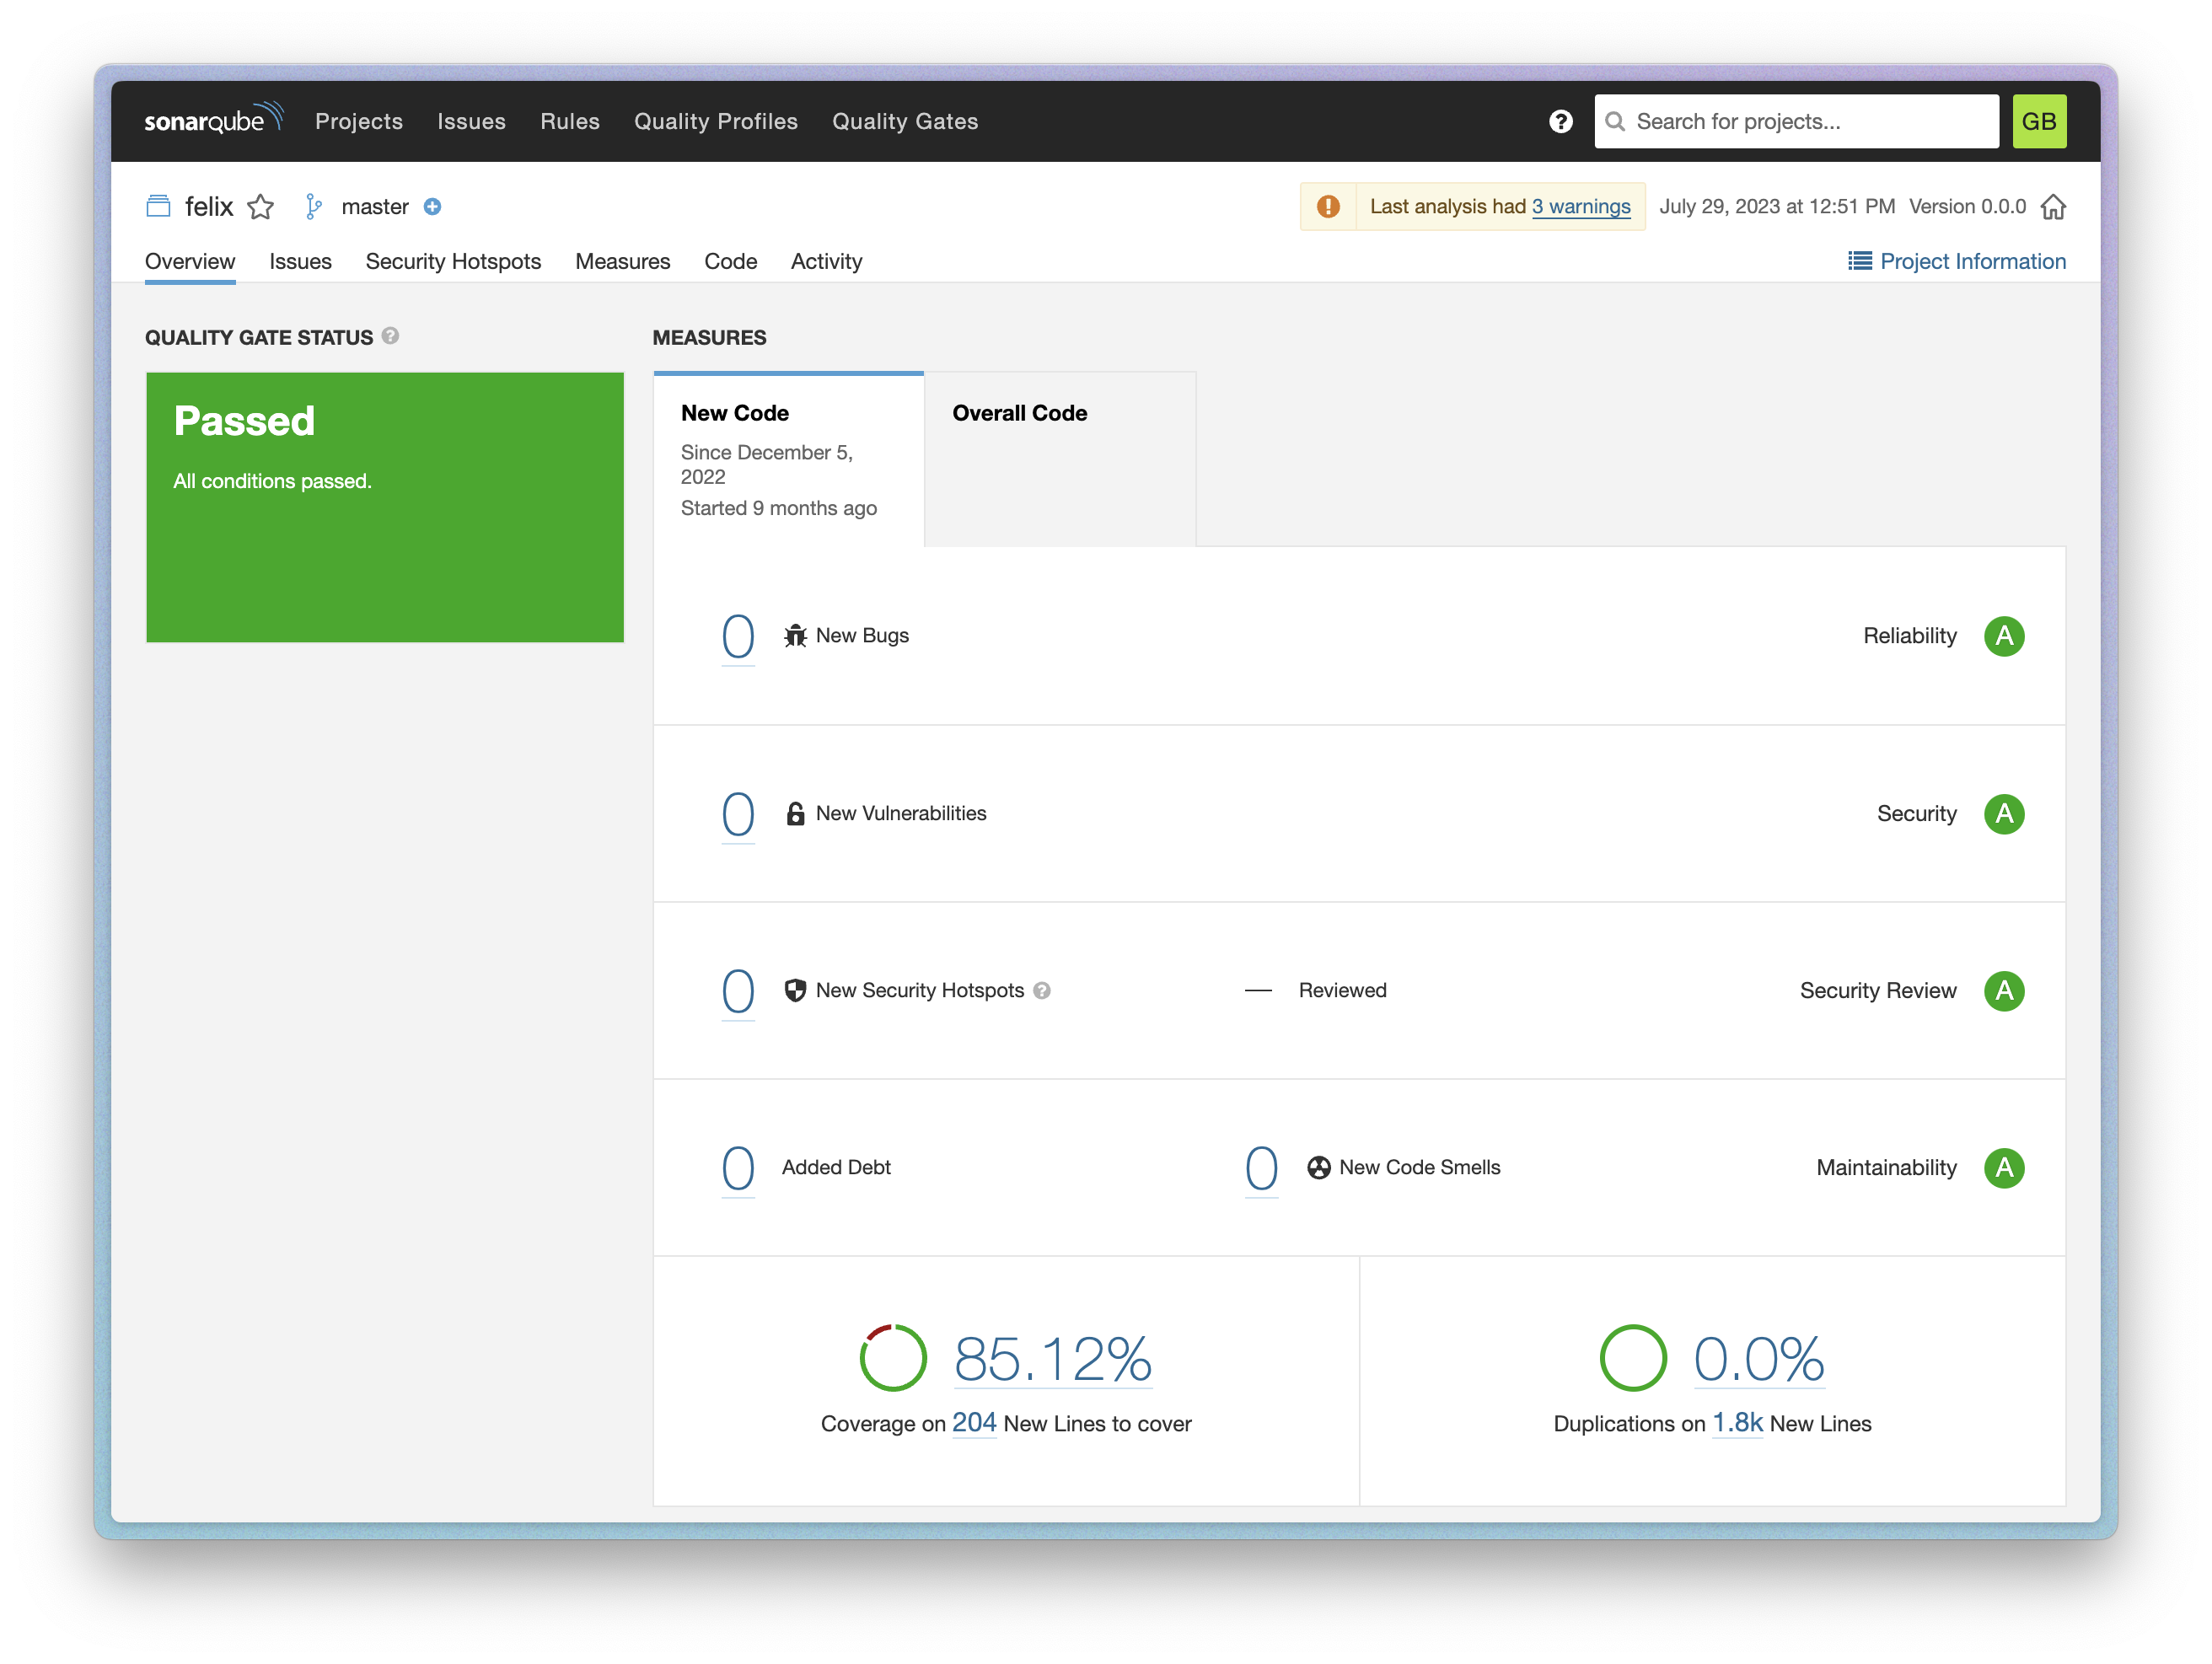
\includegraphics[height=0.70\textheight, center]{Imgs/felix-sonar.png}
    \end{column}
    \begin{column}{0.5\textwidth}
      \begin{itemize}
        \item Écriture des test unitaires et d'intégration
        \item Utilisation de librairies de mocks pour simuler certains fonctionnements
        \item Tests utilisateurs effectués à chaque fin de sprint
      \end{itemize}
    \end{column}
  \end{columns}
\end{frame}

\begin{frame}
  \frametitle{8. Mise en place d’une solution d’intégration continue}
  \begin{columns}
    \begin{column}{0.5\textwidth}
      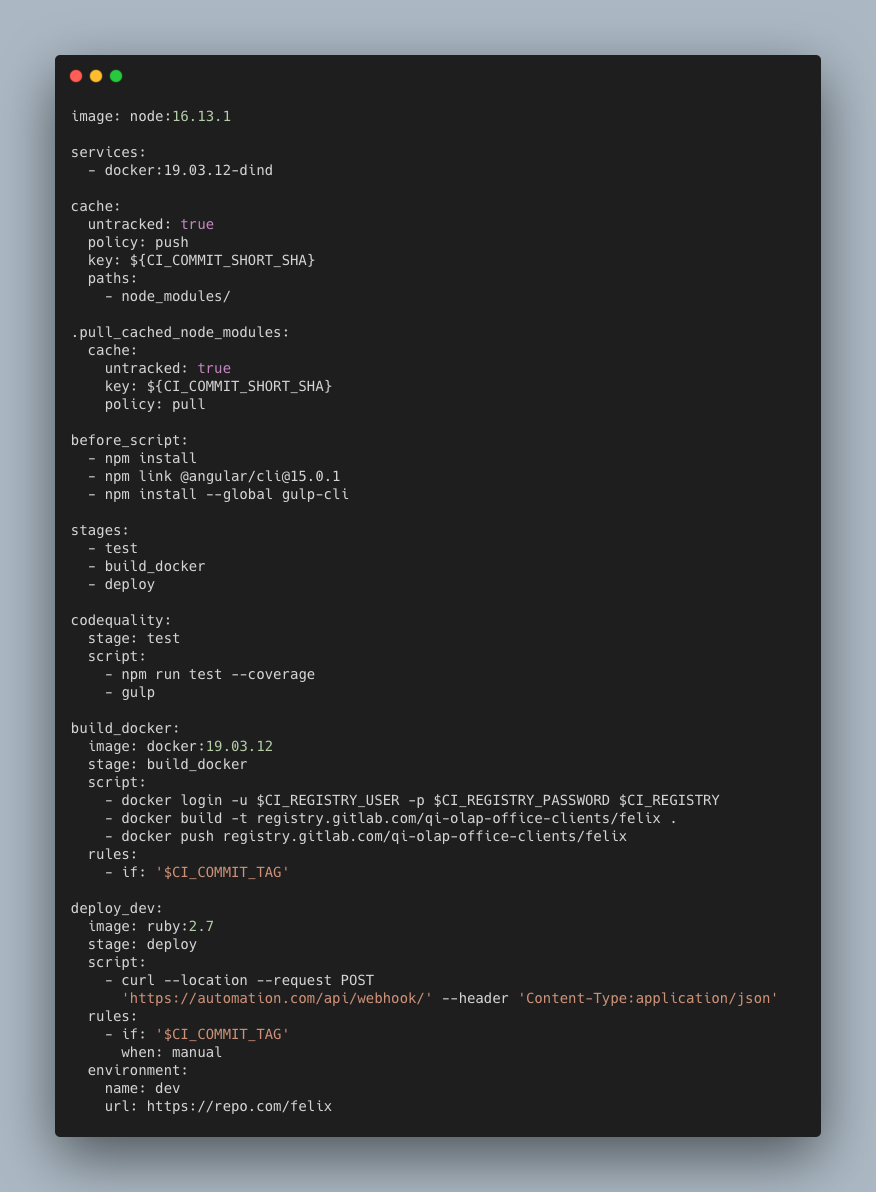
\includegraphics[height=0.75\textheight, center]{Imgs/CICD-Felix.png}
    \end{column}
    \begin{column}{0.5\textwidth}
      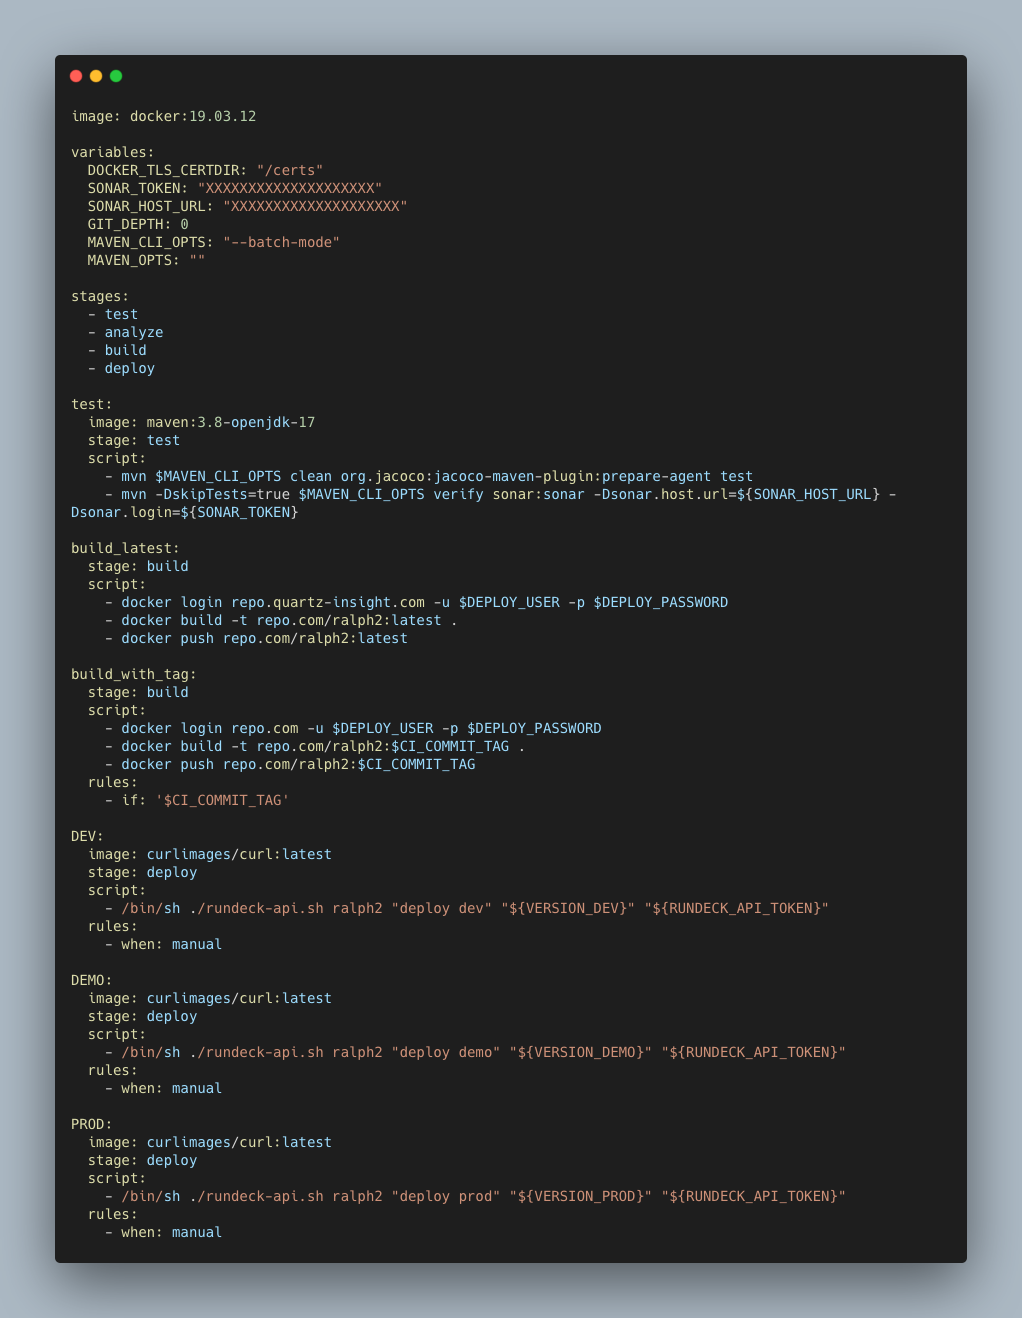
\includegraphics[height=0.75\textheight, center]{Imgs/CICD-ralph.png}
    \end{column}
  \end{columns}
\end{frame}

\begin{frame}
  \frametitle{9. Validation fonctionnelle et rédaction de la documentation pour les utilisateurs}
  \begin{columns}
    \begin{column}{0.5\textwidth}
      \begin{itemize}
        \item Documentation utilisateurs
        \item Documentation des APIs
        \item Mise en place d'un Docusaurus pour fournir la documentation
        \item la documentation pour les développeurs comme le suivi du projet
          sont sur Gitlab
      \end{itemize}
    \end{column}
    \begin{column}{0.5\textwidth}
      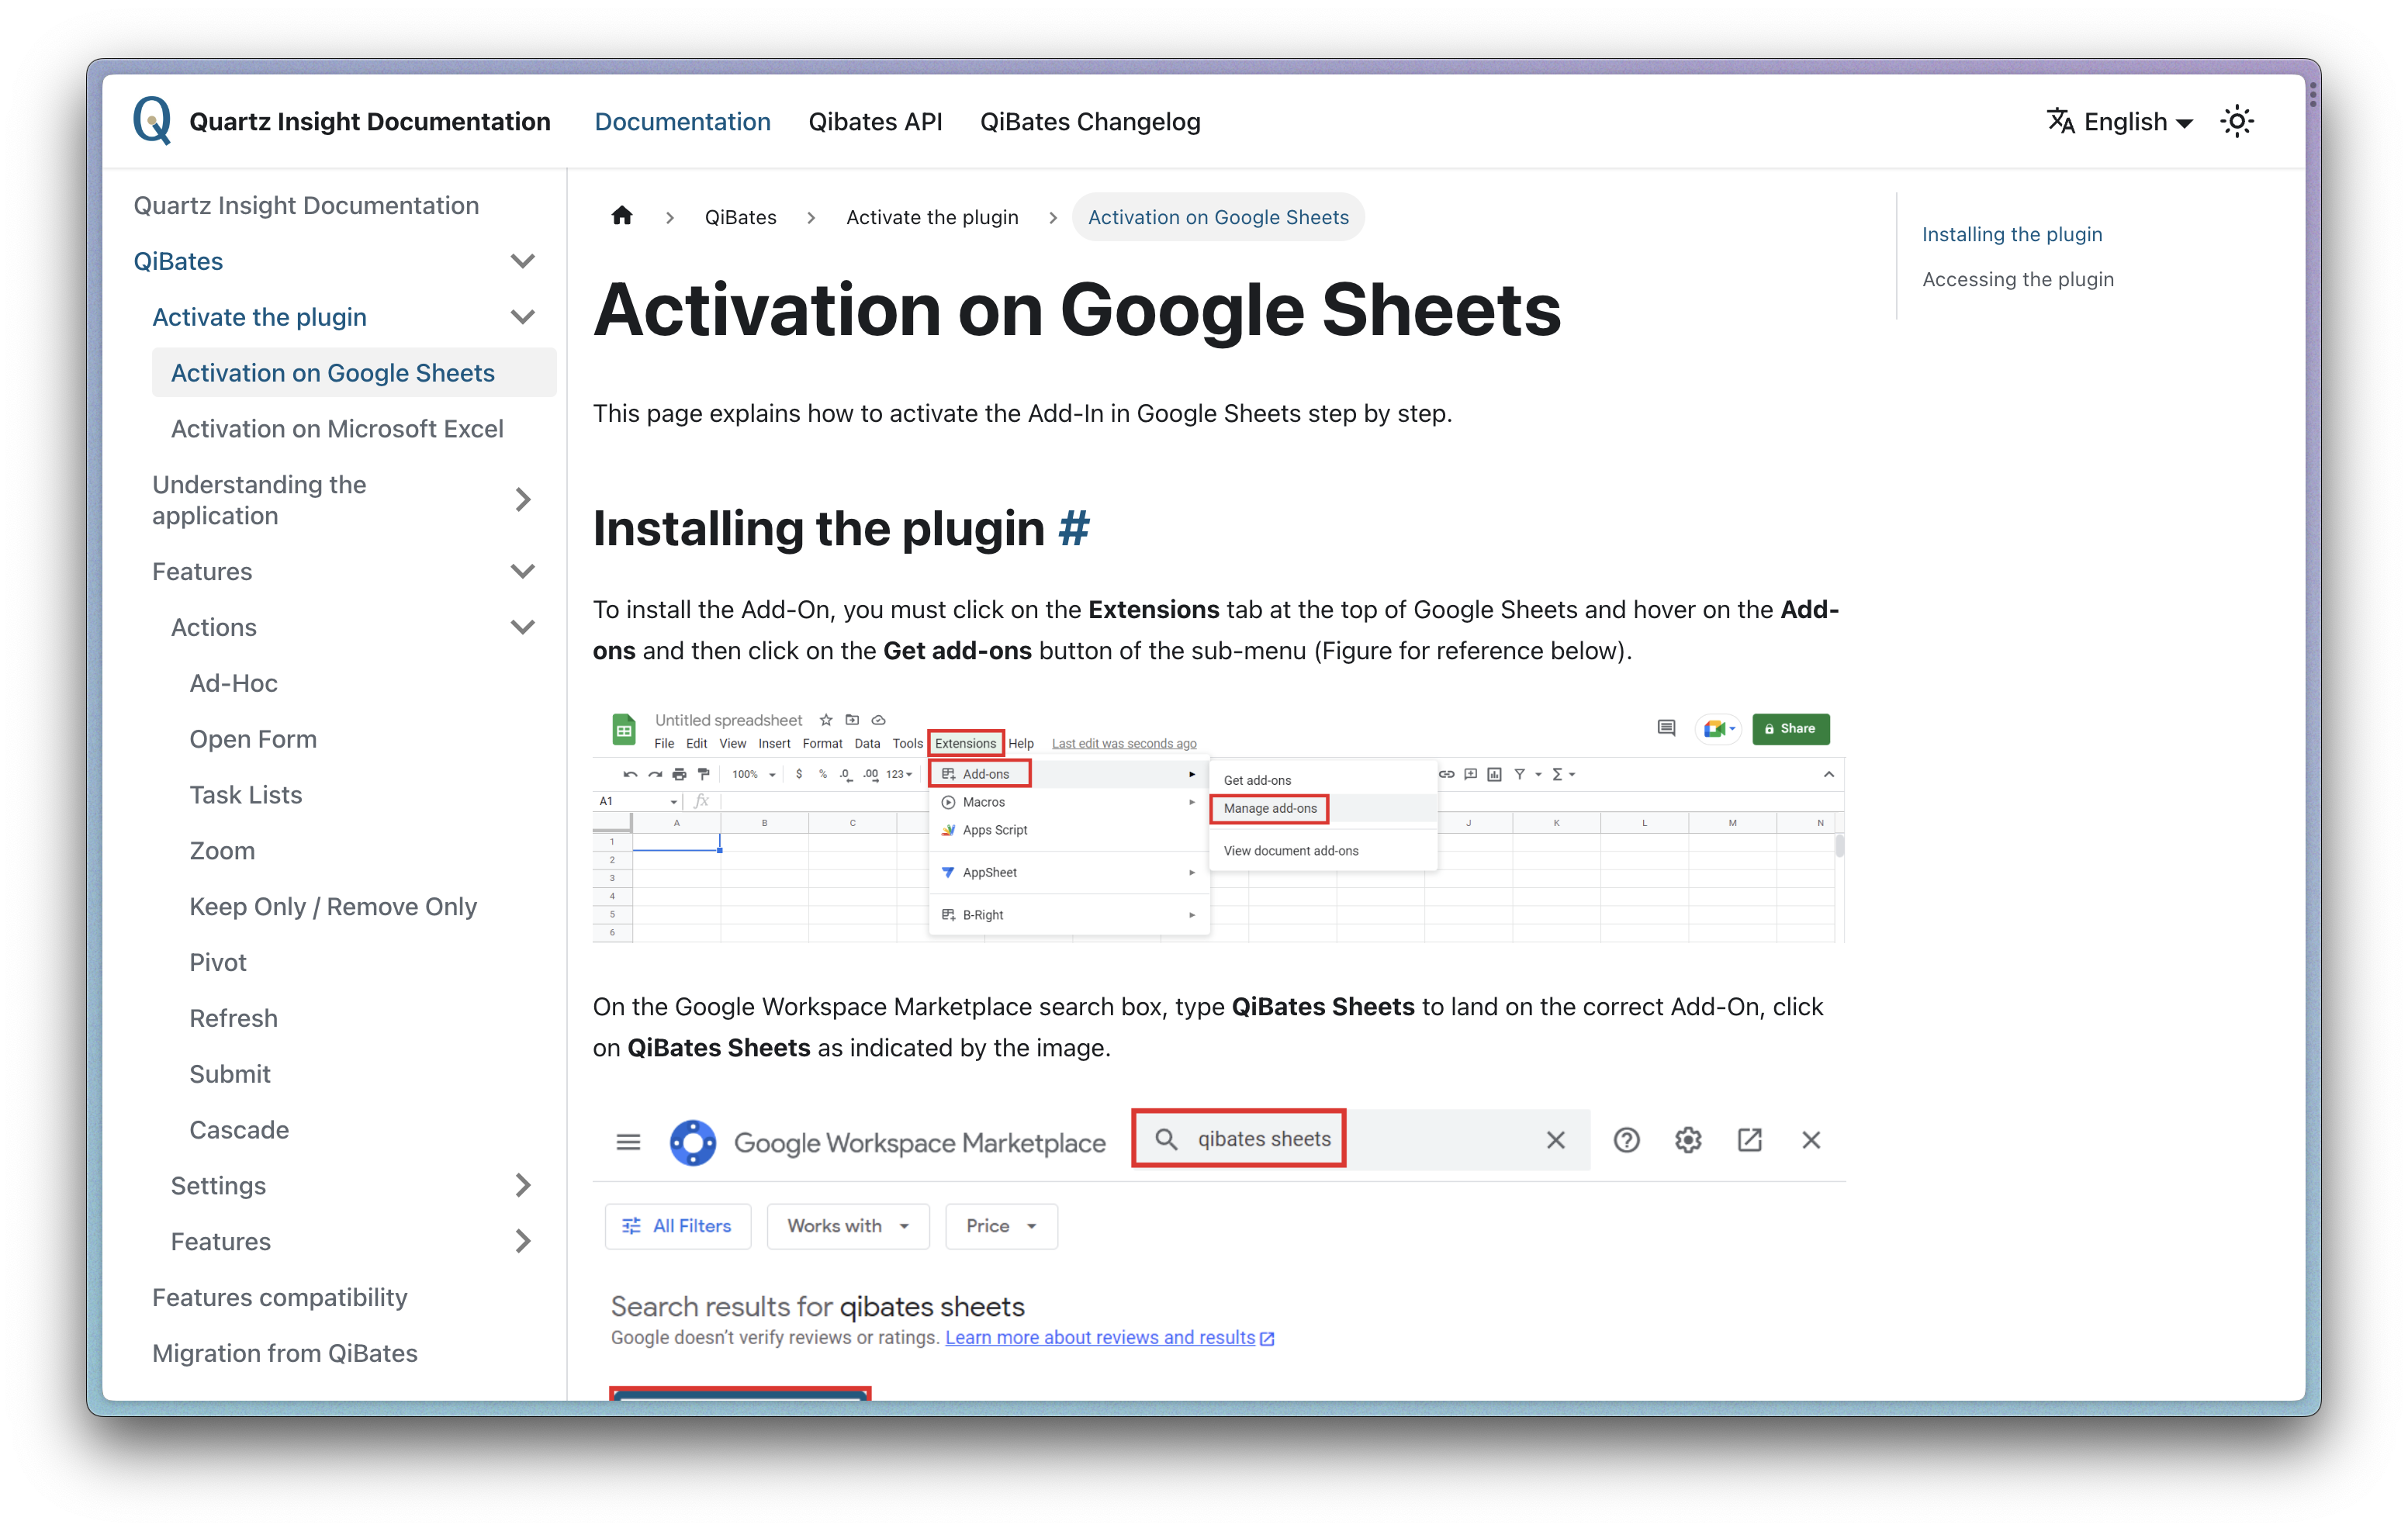
\includegraphics[height=0.60\textheight, center]{Imgs/doc-user.png}
    \end{column}
  \end{columns}
\end{frame}


\begin{frame}
  \frametitle{9. Validation fonctionnelle et rédaction de la documentation pour les utilisateurs}
  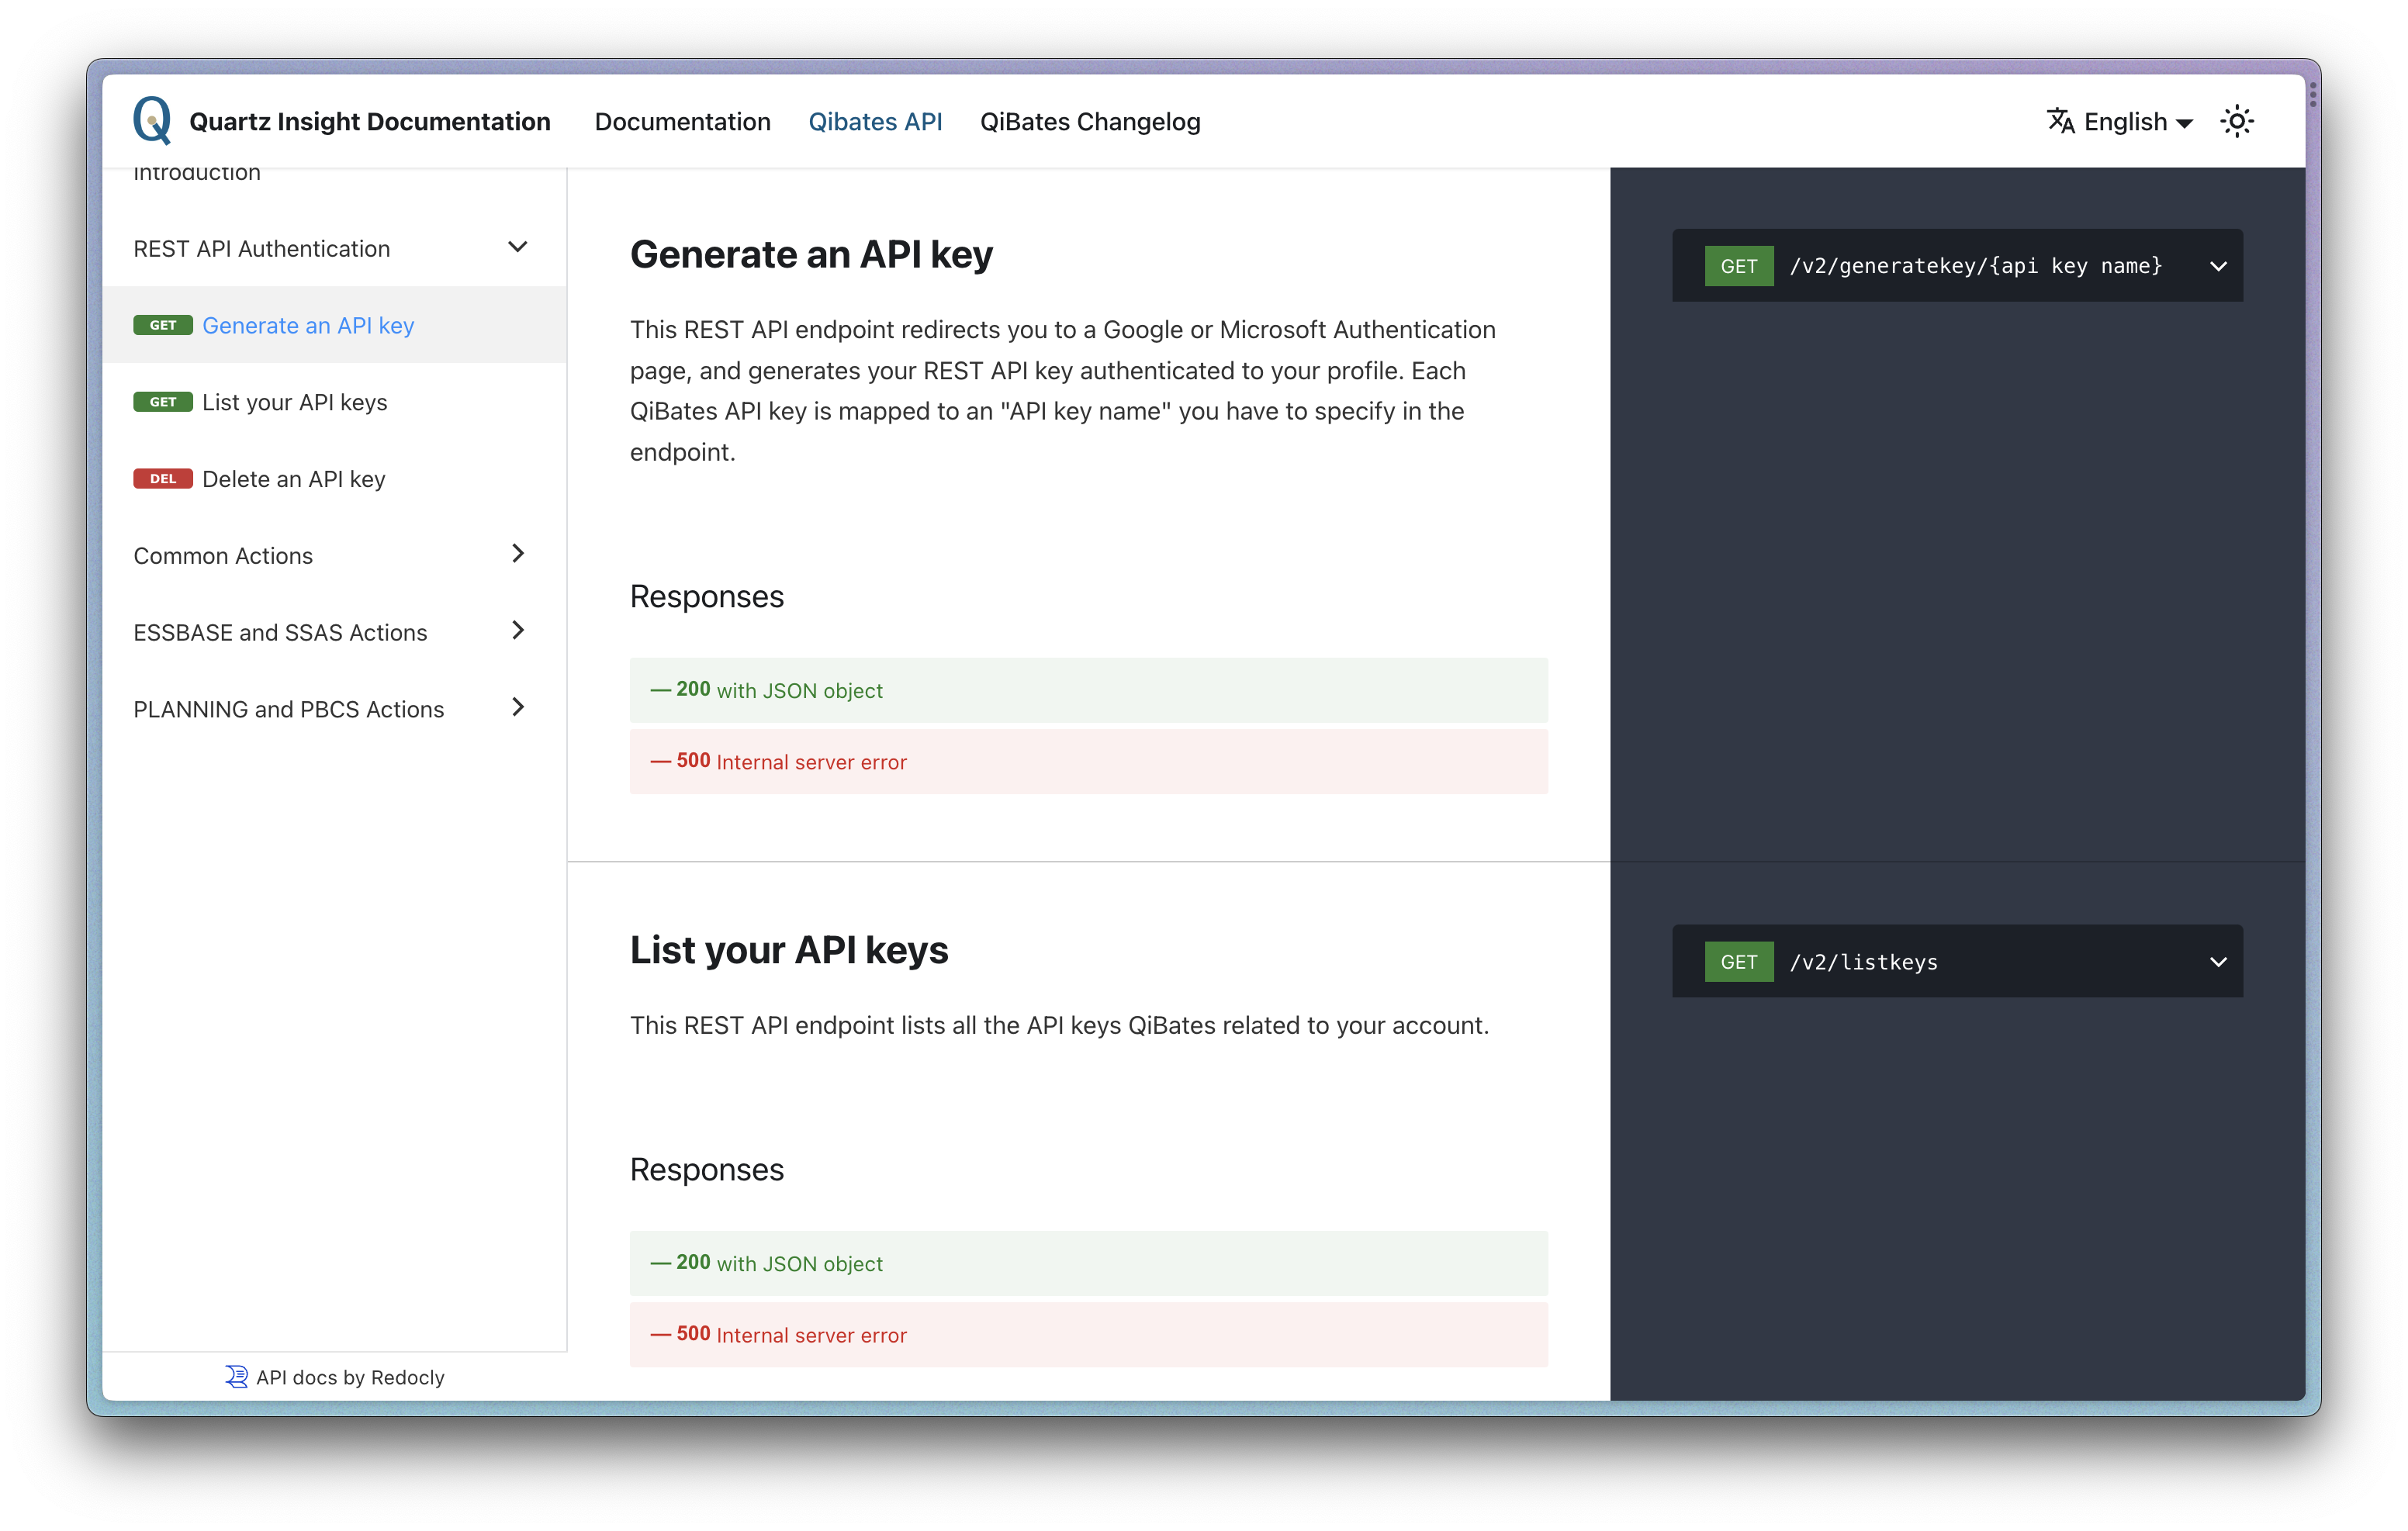
\includegraphics[height=0.80\textheight, center]{Imgs/full-doc.png}
\end{frame}

\begin{frame}
  \frametitle{10. Formation des utilisateurs, mise en place d’une enquête de satisfaction ultérieure}
  \begin{itemize}
    \item Problématiques dues au changement
    \item Modèle transitionnel de William Bridge
      \begin{itemize}
        \item 1. abandon du passé
        \item 2. zone neutre
        \item 3. nouveau départ 
      \end{itemize}
    \item Remontée de modifications pendant le développement du projet
    \item Tests et retours utilisateurs grâce à une gestion de projet agile / Scrum
  \end{itemize}
\end{frame}

\section{Conclusion}

\begin{frame}
  \frametitle{Conclusion}
  \begin{itemize}
    \item Résumé du projet
    \item L'entreprise et ses perspectives
    \item Les apports professionnels et personnels
    \item Avenir professionnel
  \end{itemize}
\end{frame}

\end{document}
